% Options for packages loaded elsewhere
\PassOptionsToPackage{unicode}{hyperref}
\PassOptionsToPackage{hyphens}{url}
%
\documentclass[
]{article}
\usepackage{amsmath,amssymb}
\usepackage{iftex}
\ifPDFTeX
  \usepackage[T1]{fontenc}
  \usepackage[utf8]{inputenc}
  \usepackage{textcomp} % provide euro and other symbols
\else % if luatex or xetex
  \usepackage{unicode-math} % this also loads fontspec
  \defaultfontfeatures{Scale=MatchLowercase}
  \defaultfontfeatures[\rmfamily]{Ligatures=TeX,Scale=1}
\fi
\usepackage{lmodern}
\ifPDFTeX\else
  % xetex/luatex font selection
\fi
% Use upquote if available, for straight quotes in verbatim environments
\IfFileExists{upquote.sty}{\usepackage{upquote}}{}
\IfFileExists{microtype.sty}{% use microtype if available
  \usepackage[]{microtype}
  \UseMicrotypeSet[protrusion]{basicmath} % disable protrusion for tt fonts
}{}
\makeatletter
\@ifundefined{KOMAClassName}{% if non-KOMA class
  \IfFileExists{parskip.sty}{%
    \usepackage{parskip}
  }{% else
    \setlength{\parindent}{0pt}
    \setlength{\parskip}{6pt plus 2pt minus 1pt}}
}{% if KOMA class
  \KOMAoptions{parskip=half}}
\makeatother
\usepackage{xcolor}
\usepackage[margin=1in]{geometry}
\usepackage{graphicx}
\makeatletter
\def\maxwidth{\ifdim\Gin@nat@width>\linewidth\linewidth\else\Gin@nat@width\fi}
\def\maxheight{\ifdim\Gin@nat@height>\textheight\textheight\else\Gin@nat@height\fi}
\makeatother
% Scale images if necessary, so that they will not overflow the page
% margins by default, and it is still possible to overwrite the defaults
% using explicit options in \includegraphics[width, height, ...]{}
\setkeys{Gin}{width=\maxwidth,height=\maxheight,keepaspectratio}
% Set default figure placement to htbp
\makeatletter
\def\fps@figure{htbp}
\makeatother
\setlength{\emergencystretch}{3em} % prevent overfull lines
\providecommand{\tightlist}{%
  \setlength{\itemsep}{0pt}\setlength{\parskip}{0pt}}
\setcounter{secnumdepth}{5}
\ifLuaTeX
  \usepackage{selnolig}  % disable illegal ligatures
\fi
\usepackage{bookmark}
\IfFileExists{xurl.sty}{\usepackage{xurl}}{} % add URL line breaks if available
\urlstyle{same}
\hypersetup{
  pdftitle={Recreating LipNet: A Simplified Approach to Lip Reading Neural Networks},
  pdfauthor={Kaleb Shah},
  hidelinks,
  pdfcreator={LaTeX via pandoc}}

\title{Recreating LipNet: A Simplified Approach to Lip Reading Neural
Networks}
\author{Kaleb Shah}
\date{2024-05-17}

\begin{document}
\maketitle

\newpage

\section{Introduction}\label{introduction}

Lip reading has gained significant attention in recent years, especially
with advancements in deep learning and artificial intelligence.
Commercially, lip reading models have potential applications in various
fields, including security, accessibility for people with hearing
impairments, and even entertainment. Celebrities, such as actors and
athletes, often find themselves at the center of gossip and intrigue,
making it valuable to capture their words even when they are not mic'd
up. Furthermore, in noisy environments, traditional speech recognition
systems can struggle, but lip reading models can provide additional
context to enhance accuracy.

In this project, inspired by the original LipNet paper by Assael et
al.~(2016), I aimed to recreate a simplified version of the LipNet
model. My goal was to determine if such models could be made lightweight
and developed with fewer resources while maintaining a reasonable level
of accuracy. The original LipNet implementation was in TensorFlow,
whereas I have utilized PyTorch for my implementation. By doing so, I
tested the reproducibility of the paper across different technologies.

Beyond commercial applications, lip reading technology has profound
implications for accessibility. Individuals with hearing impairments
could greatly benefit from augmented reality (AR) lenses and virtual
reality (VR) goggles equipped with lip reading capabilities. Such
technology could transcribe speech to text in real-time, providing an
invaluable tool for communication in various settings. Moreover,
combining lip reading models with speech recognition systems could
enhance performance in noisy environments, thus broadening the scope of
practical applications.

My simplified LipNet model focuses on sentence-level lip reading,
following the structure of the original LipNet, which maps a sequence of
video frames to text using spatiotemporal convolutions, a recurrent
network, and connectionist temporal classification (CTC) loss. The
original LipNet achieved a remarkable 95.2\% accuracy on the GRID
corpus, significantly outperforming human lip readers. In my project, I
aimed to replicate this success to a certain extent, albeit with reduced
computational resources and simpler architecture.

The structure of this report is as follows: the Methods section details
my approach to model design, data preparation, and training. The Results
section presents the performance metrics of my model, and the Discussion
section compares my findings with the original LipNet model and
addresses the limitations of my approach. Finally, the References
section lists the sources that informed my work.

\section{Methods}\label{methods}

The dataset used in this project is the Lombard Grid corpus, a bi-view
audiovisual Lombard speech corpus designed for joint
computational-behavioral studies in speech perception. It includes 54
talkers with 1000 utterances per talker, following the same sentence
format as the audiovisual Grid corpus but with unique sentence sets. For
the scope of this project, I focused on one speaker to simplify the
analysis and manage computational resources.

To prepare the data, video frames were loaded using the OpenCV library.
Code for this processing was adapted by Nick Nochnack's Tensorflow
Implementation of LipNet (in References). Each frame was converted to
grayscale to reduce computational complexity and then cropped to focus
on the mouth region, ensuring that the model learns relevant features
(Appendix - Figure 7). The frames were converted to PyTorch tensors and
normalized by subtracting the mean and dividing by the standard
deviation, ensuring uniformity in pixel intensity values (Appendix -
Figure 8). To handle variable-length sequences, frames were padded to
create uniform-length sequences using PyTorch's \texttt{pad\_sequence}
function. Alignments were loaded and tokenized using a custom character
mapping, encoding each character in the sentences to a numerical index,
including a padding token to handle variable-length text sequences. Data
was batched using a DataLoader with a custom collate function to pad
both frames and alignments appropriately.

There are two model architectures in this paper. The primary one follows
the original LipNet but with a few modifications to simplify the
implementation using PyTorch. The model starts with three layers of 3D
convolutions to capture spatiotemporal features from the video frames.
Each convolutional layer is followed by a max-pooling layer to reduce
the spatial dimensions, thereby managing computational load and focusing
on essential features. The features extracted by the convolutional
layers are then passed to two bidirectional GRU (Gated Recurrent Unit)
layers. GRUs are well-suited for temporal data as they can capture
dependencies over time.The bidirectional nature of these layers allows
the model to access both past and future context, improving the accuracy
of the predictions. The output from the GRU layers is fed into a fully
connected linear layer followed by a softmax layer to generate
probability distributions over the character set at each time step. The
secondary model is exactly the same but with only one GRU layer.

For optimization, I used the Adam optimizer, known for its efficient
handling of sparse gradients and adaptive learning rate capabilities.
This optimizer helps in faster convergence and better performance. The
Connectionist Temporal Classification (CTC) loss function was used for
training. CTC is ideal for sequence prediction tasks with
variable-length outputs as it does not require pre-segmented training
data, making it suitable for lip reading where the alignment between
video frames and text is not explicitly available. The CTC loss function
calculates the probability of the correct label sequence by summing over
all possible alignments, which allows the model to learn from unaligned
data effectively.

To enhance the training process, a learning rate scheduler was
implemented to reduce the learning rate gradually. This helps the model
converge more smoothly by preventing the learning rate from being too
high, which could cause the model to overshoot the optimal parameters.
The scheduler decreases the learning rate after a certain number of
epochs or based on the validation loss, ensuring more stable
convergence.

In addition to the main processing steps, I incorporated a
post-processing phase to further refine the model's predictions using
the TextBlob library. This phase was essential to correct spelling
errors and normalize the predicted text sequences. Given that typical
alignments in my dataset rarely exceed 30 characters since the mean
length is 24.83 characters, I implemented a character limit to ensure
the efficiency and relevance of the post-processed output. TextBlob was
used to correct any apparent spelling mistakes in the raw predictions.
The corrected text was then tokenized, and tokens were concatenated
until the 30-character limit was reached. This limit was based on the
average length of the sentences in the Lombard Grid corpus, ensuring
that the post-processed text remained concise and relevant to the
original input. Thus enhancing the accuracy of the final predictions.

For evaluation, I used two primary metrics: edit distance and word
coverage. Edit distance, specifically Levenshtein distance, measures the
number of insertions, deletions, and substitutions required to transform
the predicted sequence into the ground truth. This metric provides a
robust measure of the model's accuracy in predicting the correct
sequence of characters. Word coverage quantifies the fraction of words
from the original text that are correctly predicted in the output. It is
calculated by dividing the number of correct words by the total number
of words in the ground truth. While word coverage captures the amount of
information retained, it does not account for additional incorrect words
in the prediction, which can sometimes give an incomplete picture of the
model's performance.

\section{Results}\label{results}

Initially, it is important to note that these results are based on
in-sample predictions due to oversights during the experiments, which
will be addressed later.

I began by training the model with just one GRU layer. The loss curve
for this model is shown in Figure 2 in the appendix. During training, I
observed that the loss oscillated between 1.6 and 1.7 across epochs
instead of steadily decreasing. This indicated potential issues with the
model's capacity to learn from the data effectively. Consequently, I
decided to add an additional GRU layer, thereby aligning the model more
closely with the original LipNet architecture.

As shown in Figure 3 of the appendix, the two-layer GRU model, despite
starting with a higher initial cost than the single-layer model,
exhibited a lower loss by the 10th epoch. This improvement is visually
evident in Figure 4, where the cost curves for both models intersect at
the 7th epoch. The two-layer GRU model demonstrated a more consistent
decrease in loss, which motivated us to adopt this architecture for
further training.

I continued training the two-layer GRU model for a total of 100 epochs.
Over this period, the loss decreased from over 2.5 to approximately 0.2,
showcasing the model's learning capability as seen in Figure 1 and 10 of
the Appendix. However, due to computing limitations, further training
beyond 100 epochs was not feasible. These limitations and their
implications will be discussed in a later section.

The predictions generated by my model were evaluated using the average
edit distance, which was found to be 4.887. Given the mean sequence
length of 24.83 characters, this indicates that on average, 4.887
character changes (insertions, deletions, or substitutions) are needed
to achieve 100\% accuracy. The distribution of accurate predictions at
different edit distances can be found in Figure 5 of the Appendix.
Post-processing with TextBlob significantly improved the predictions,
reducing the average edit distance by 11.22, detailed in figure 6 in the
appendix. This reduction was primarily due to the trimming of trailing
noise in the predictions, which was often introduced by padding
sequences to a uniform length of 40 characters.

I also evaluated the model's performance at various edit distance
thresholds. The cumulative accuracy increased with the allowance of more
edits, as illustrated in Figure 5 and 9 of the appendix. With zero
edits, 8.2\% of the predictions achieved 100\% accuracy. At an edit
distance of two, 23.2\% of the predictions were accurate, while an edit
distance of six resulted in 52.4\% accuracy. The accuracy plateaued at
91.7\% with an edit distance of nine.

Furthermore, the average word coverage, which measures the fraction of
words from the original text correctly predicted in the output, was
78.28\%. This metric indicates that while the model captures a
significant portion of the original information, there is still room for
improvement, particularly in minimizing extraneous words and refining
the accuracy of the predicted text.

Overall, these results highlight the model's capability to learn and
improve over time, the effectiveness of adding an additional GRU layer,
and the benefits of post-processing. The observed limitations and
potential areas for future improvements will be addressed in the
following sections.

\section{Discussion}\label{discussion}

In this project, I aimed to recreate a simplified version of LipNet, a
model for sentence-level lip reading. There are several differences
between my model and the original LipNet presented by Assael et
al.~(2016). Firstly, while the original LipNet was implemented in
TensorFlow, my version uses PyTorch, providing a different framework for
model development. Additionally, the original LipNet utilized a more
complex architecture with higher computational power and resources,
while my model was intentionally simplified to test its feasibility with
fewer resources. I also focused on a single speaker from the Lombard
Grid corpus, using only the front view, whereas the original model used
a more diverse dataset with multiple speakers and bi-view including
front and side configurations.

My approach faced several limitations, particularly concerning the
in-sample data. Due to an oversight, the data loader was not saved,
preventing the replication of the exact training and testing splits.
Moreover, working on Google Colab for increased computational power
introduced challenges. During one session, I was kicked out, leading to
the loss of the train-test split since it was randomly generated. This
disruption meant the model was only trained on the training data without
a separate test set for evaluation, limiting the robustness of my
results.

The project primarily aimed to test the reproducibility of existing
technologies. By focusing on one speaker and only using the front view,
my findings are not generalizable beyond the Lombard Grid corpus. The
character count limitation, with alignments averaging 24 characters,
poses another restriction; the model's performance on longer sequences
remains untested. Additionally, my model showed an over-reliance on
post-processing with TextBlob. While this step significantly improved
the predictions, it indicates that the raw model outputs were less
accurate, and such heavy reliance on post-processing might not be ideal
in practical applications.

Training beyond 100 epochs would require purchasing more computational
resources, which was not feasible within the scope of this project. This
limitation highlights the need for more powerful hardware to further
enhance the model's performance and reduce the loss beyond the achieved
levels.

Ethical and privacy concerns also arise with lip-reading technologies.
The ability to read lips without consent can lead to significant privacy
violations, particularly for individuals who are unaware that their
speech is being transcribed. This raises important questions about the
responsible use of such technologies and the need for clear regulations
and ethical guidelines to protect individuals' privacy.

To conclude, this project demonstrates the potential for reproducing
complex models like LipNet on a smaller scale, highlighting both the
possibilities and the challenges. Future work should address the
limitations discussed, explore generalizability to broader datasets, and
consider the ethical implications of deploying lip-reading technologies
in real-world scenarios.

\newpage

\section{References}\label{references}

Assael, Y. M., Shillingford, B., Whiteson, S., \& de Freitas, N. (2016).
LipNet: End-to-End Sentence-Level Lipreading. arXiv preprint
arXiv:1611.01599. Retrieved from \url{https://arxiv.org/abs/1611.01599}

``Build a Deep Learning Model that can LIP READ using Python and
Tensorflow Full Tutorial.'' YouTube, uploaded by Nick Nochnack, 29
Apr.~2024, www.youtube.com/watch?v=uKyojQjbx4c.

\newpage

\section{Appendix}\label{appendix}

\begin{figure}
\centering
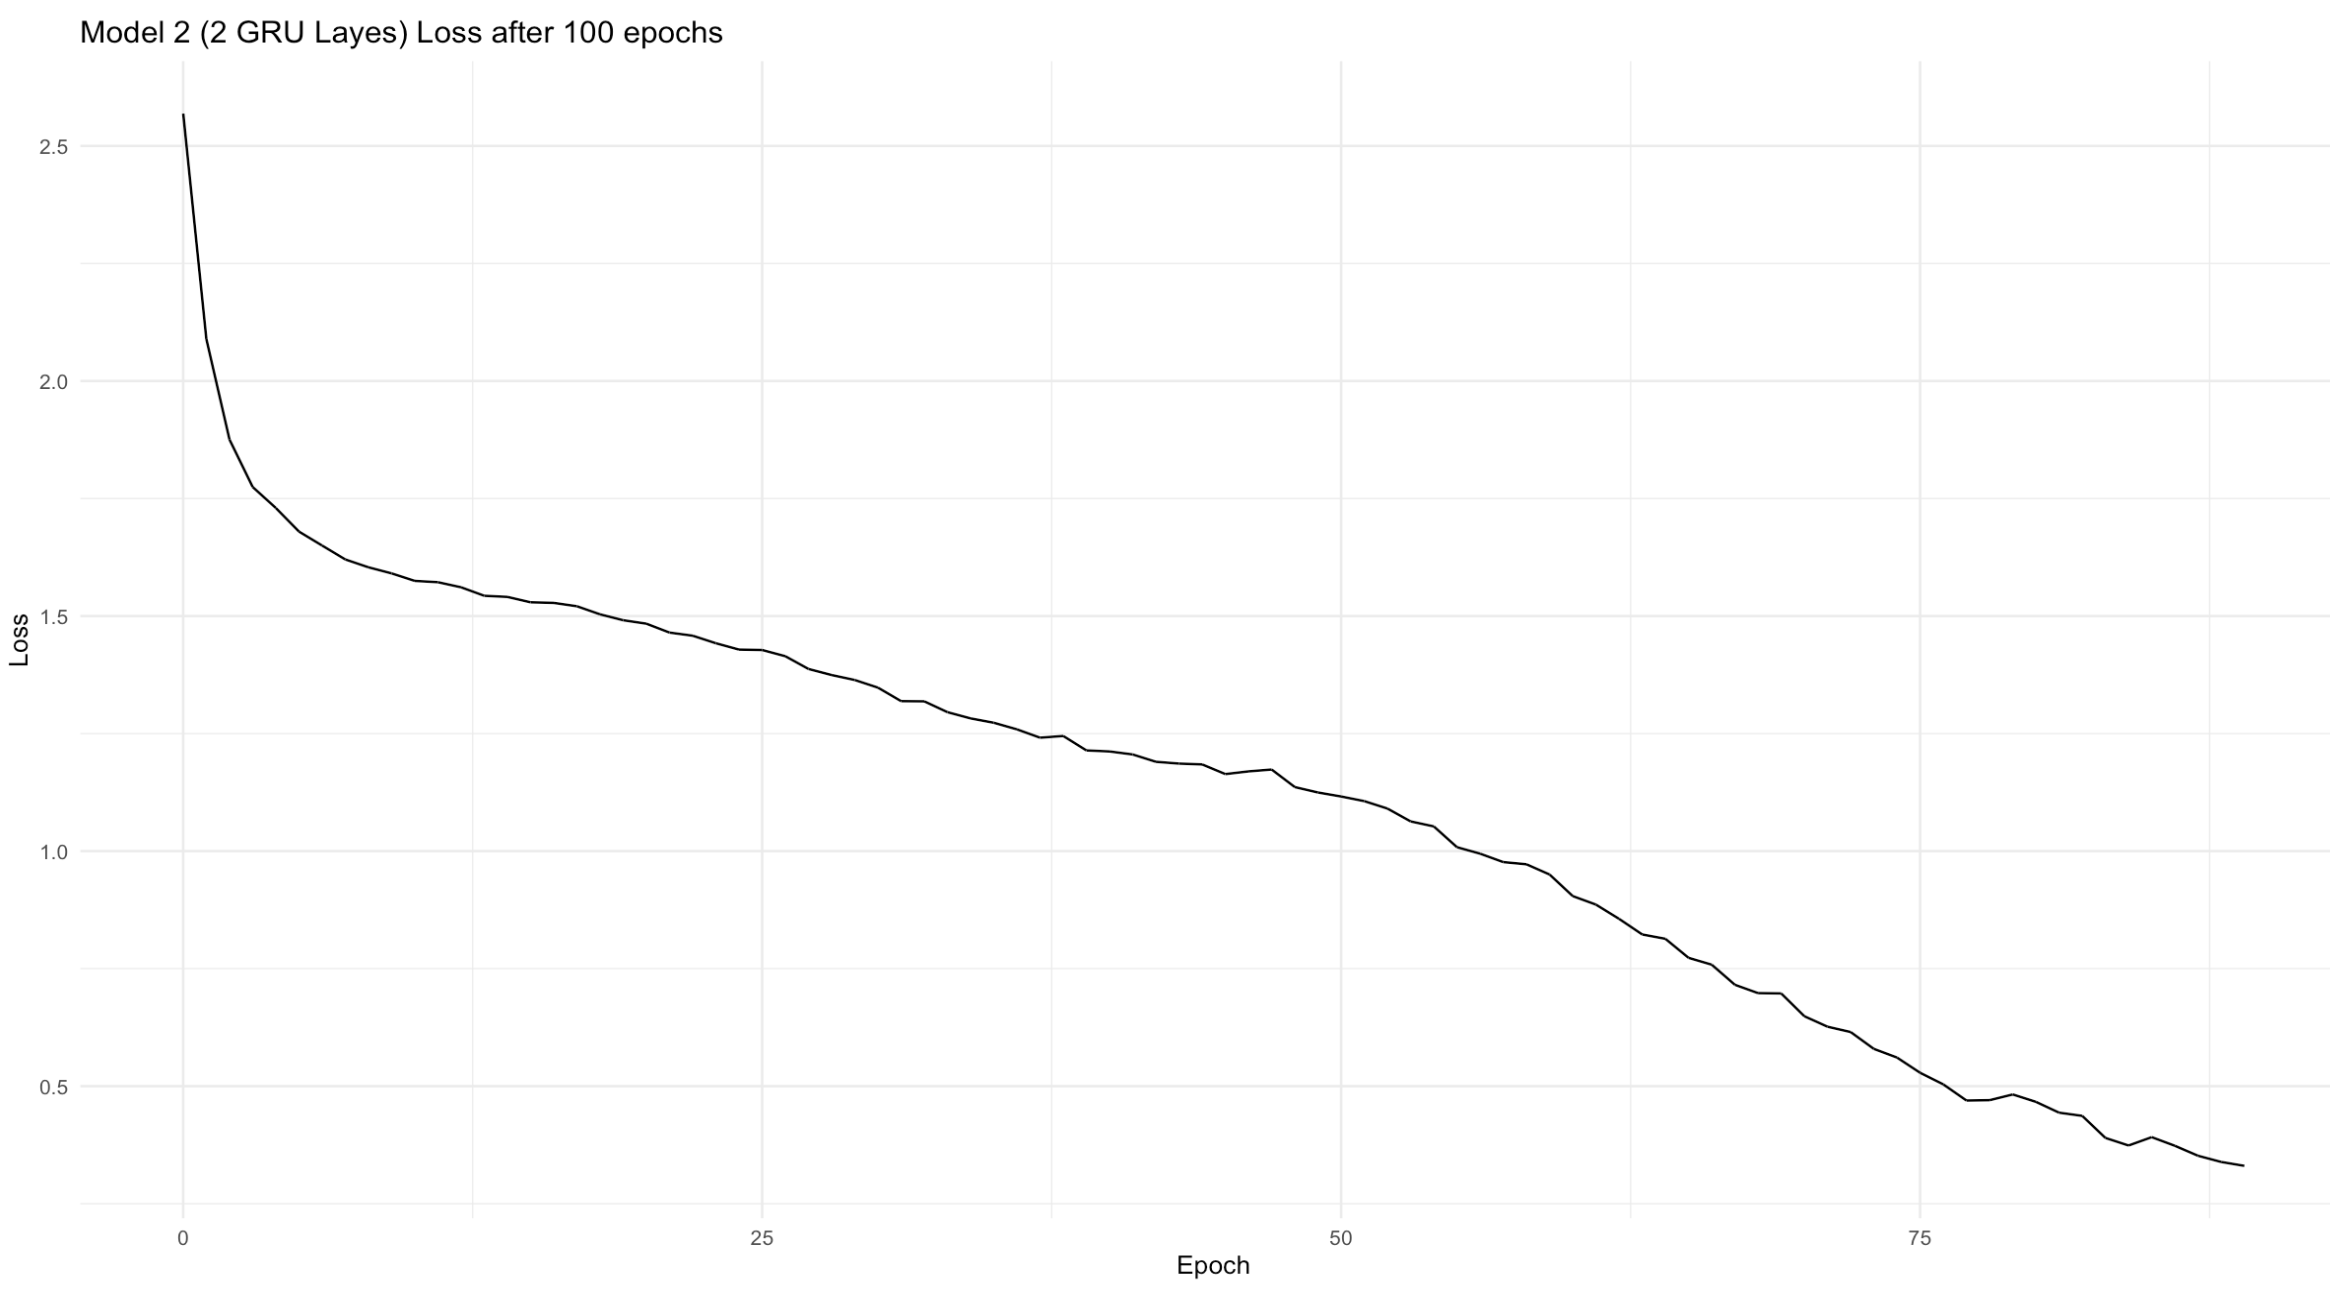
\includegraphics{"../Figures/Figure_1.png"}
\caption{Figure 1}
\end{figure}

\begin{figure}
\centering
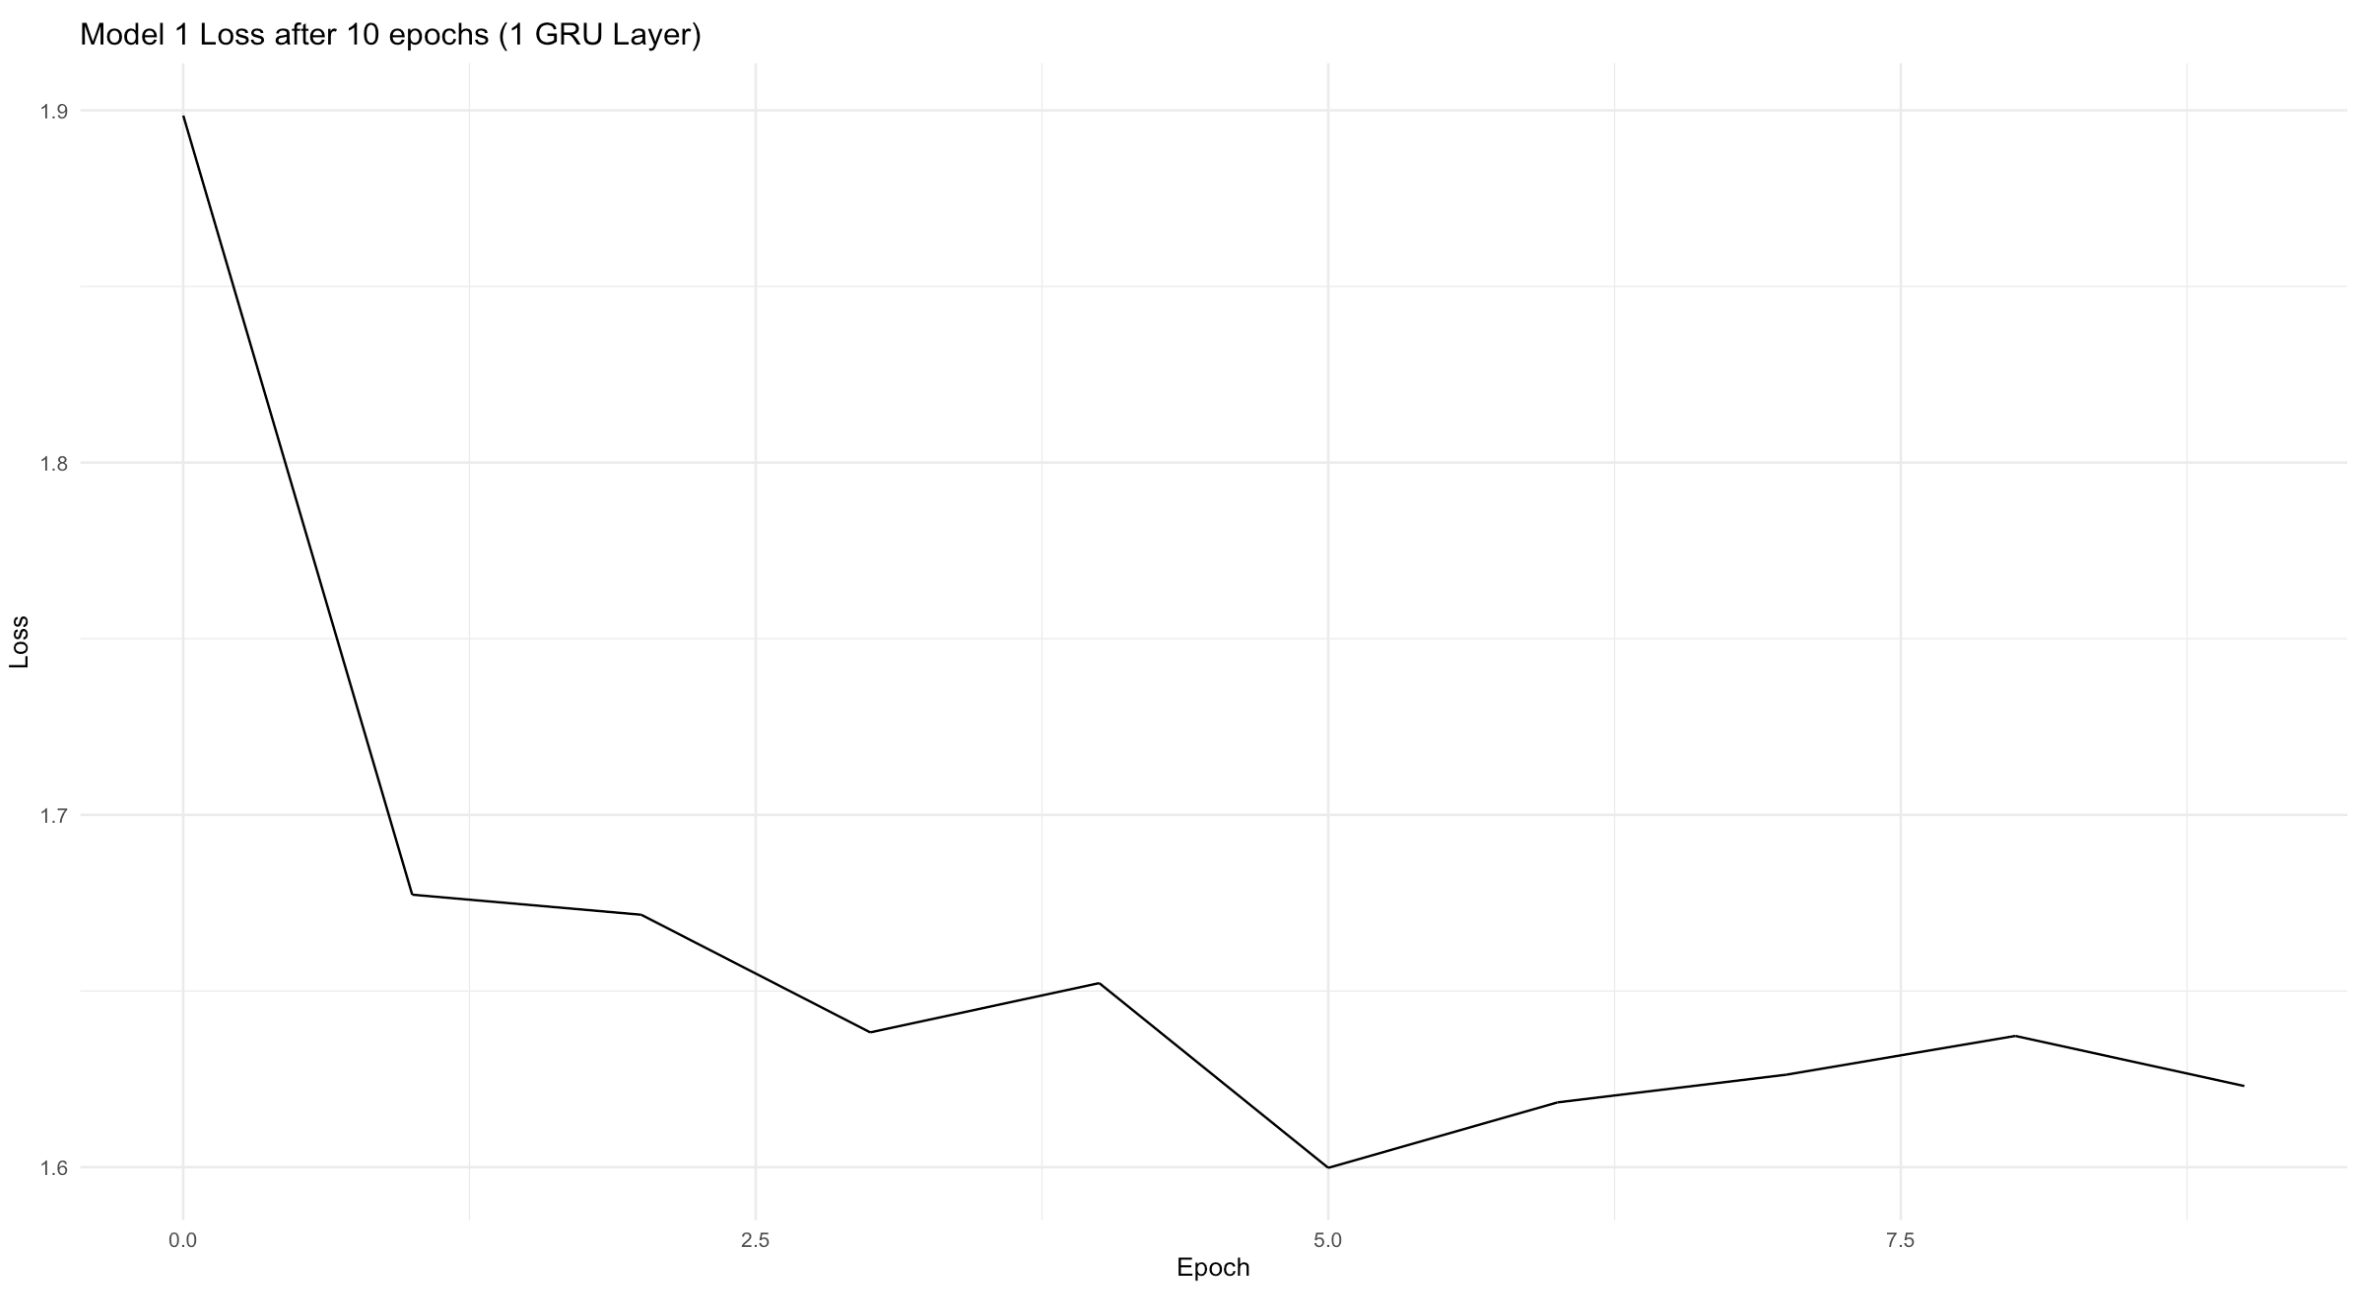
\includegraphics{"../Figures/Figure_2.png"}
\caption{Figure 2}
\end{figure}

\begin{figure}
\centering
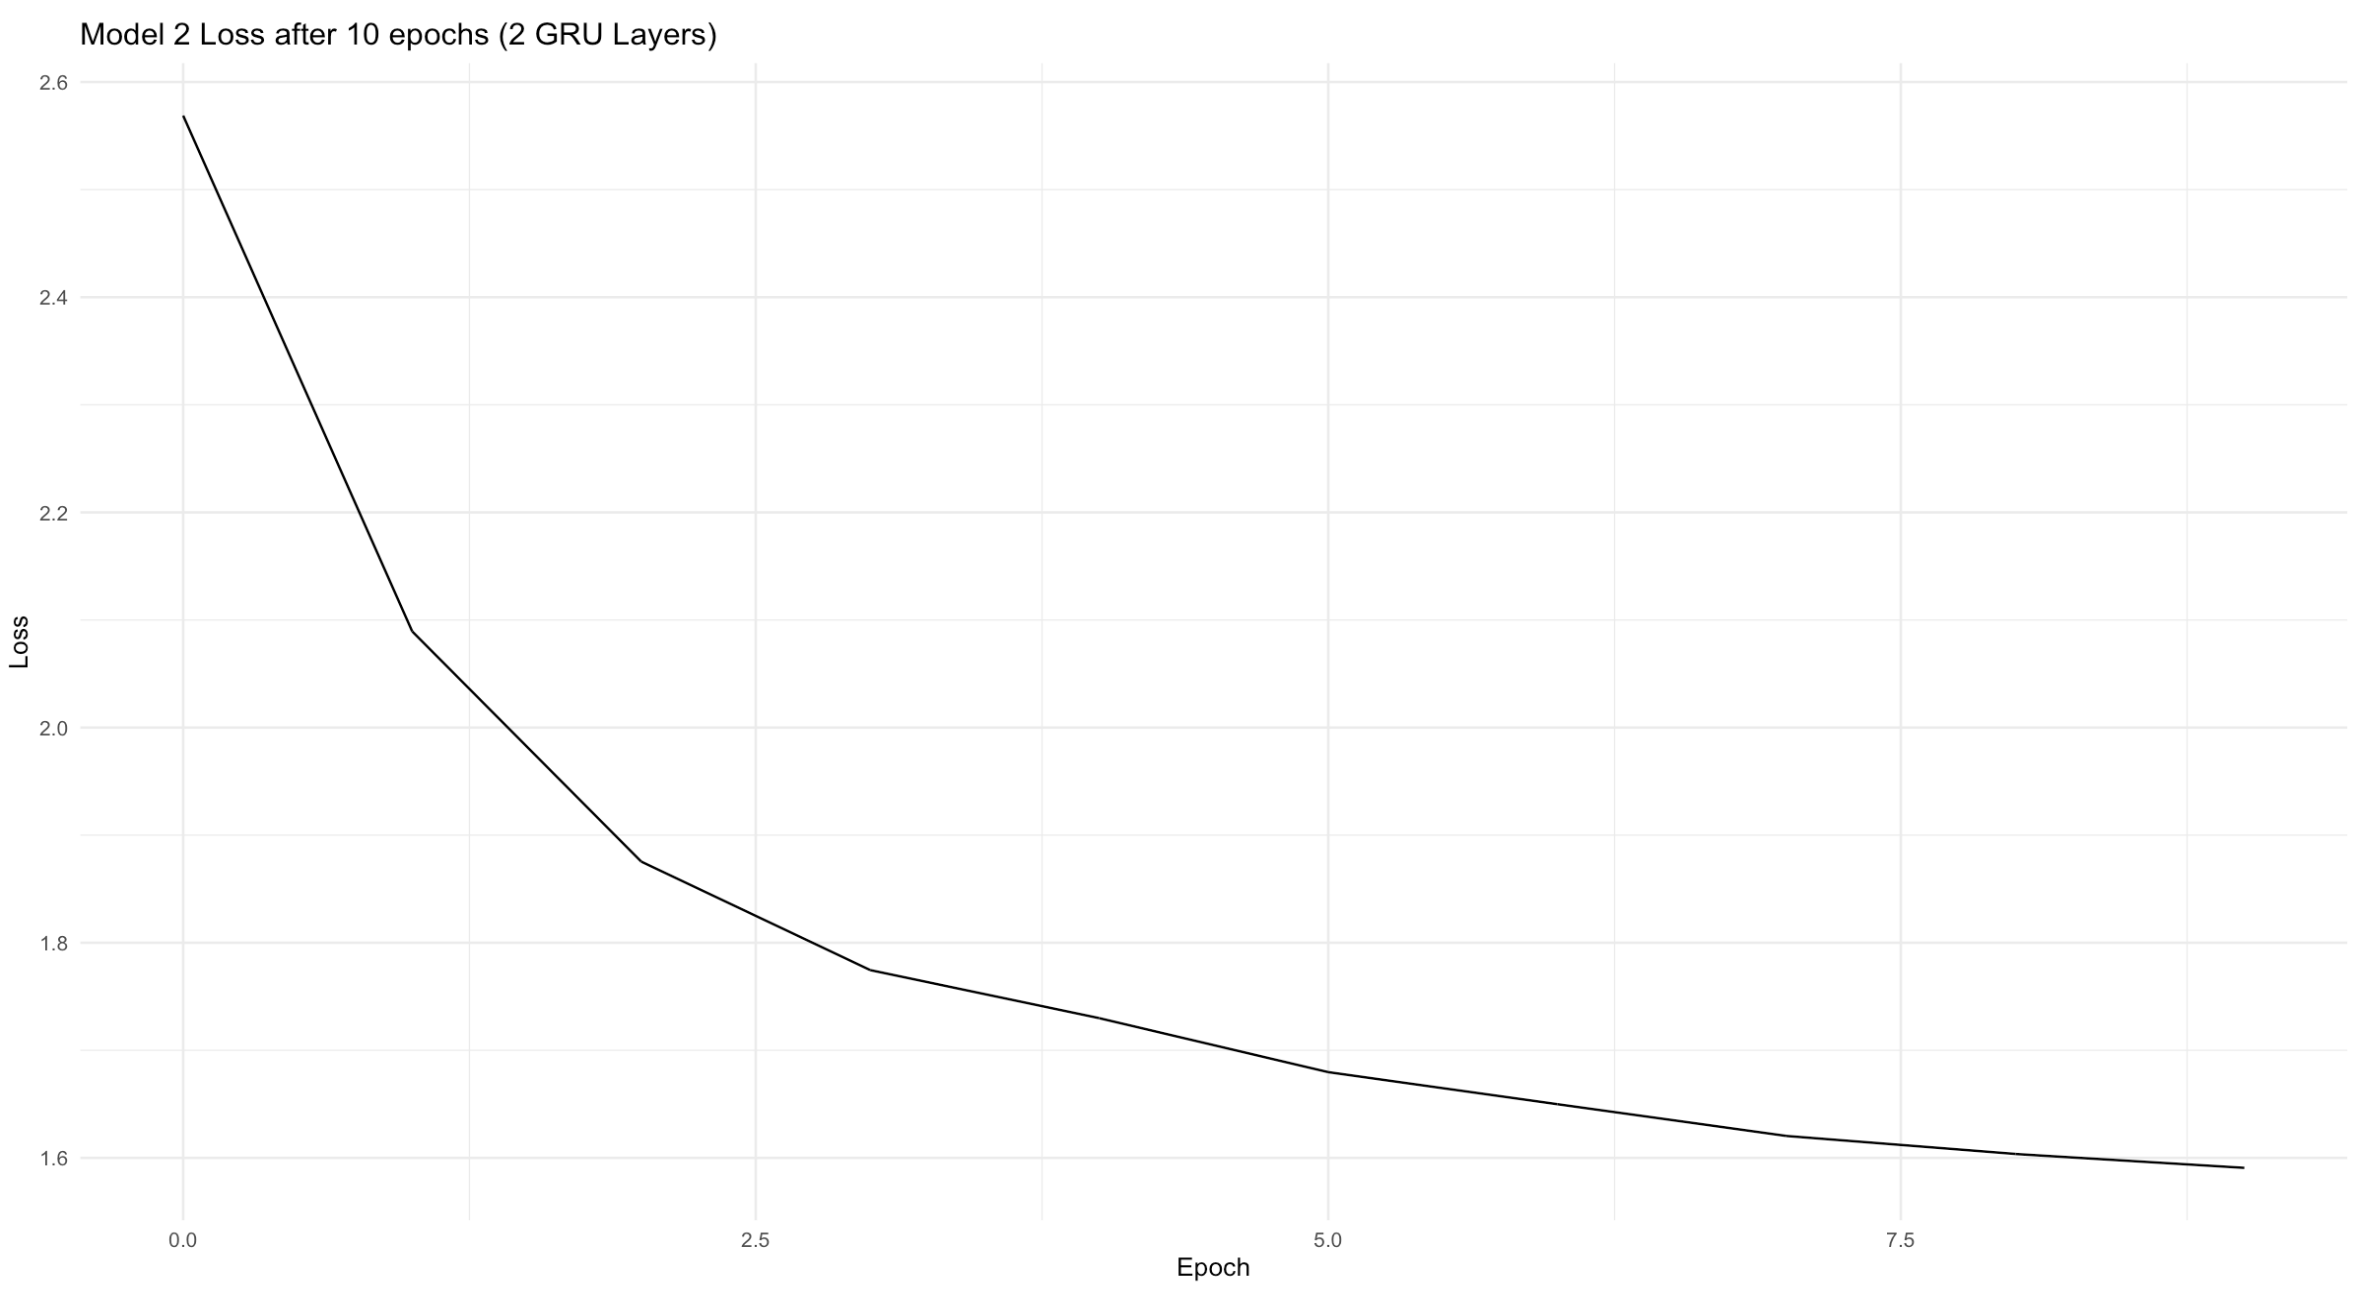
\includegraphics{"../Figures/Figure_3.png"}
\caption{Figure 3}
\end{figure}

\begin{figure}
\centering
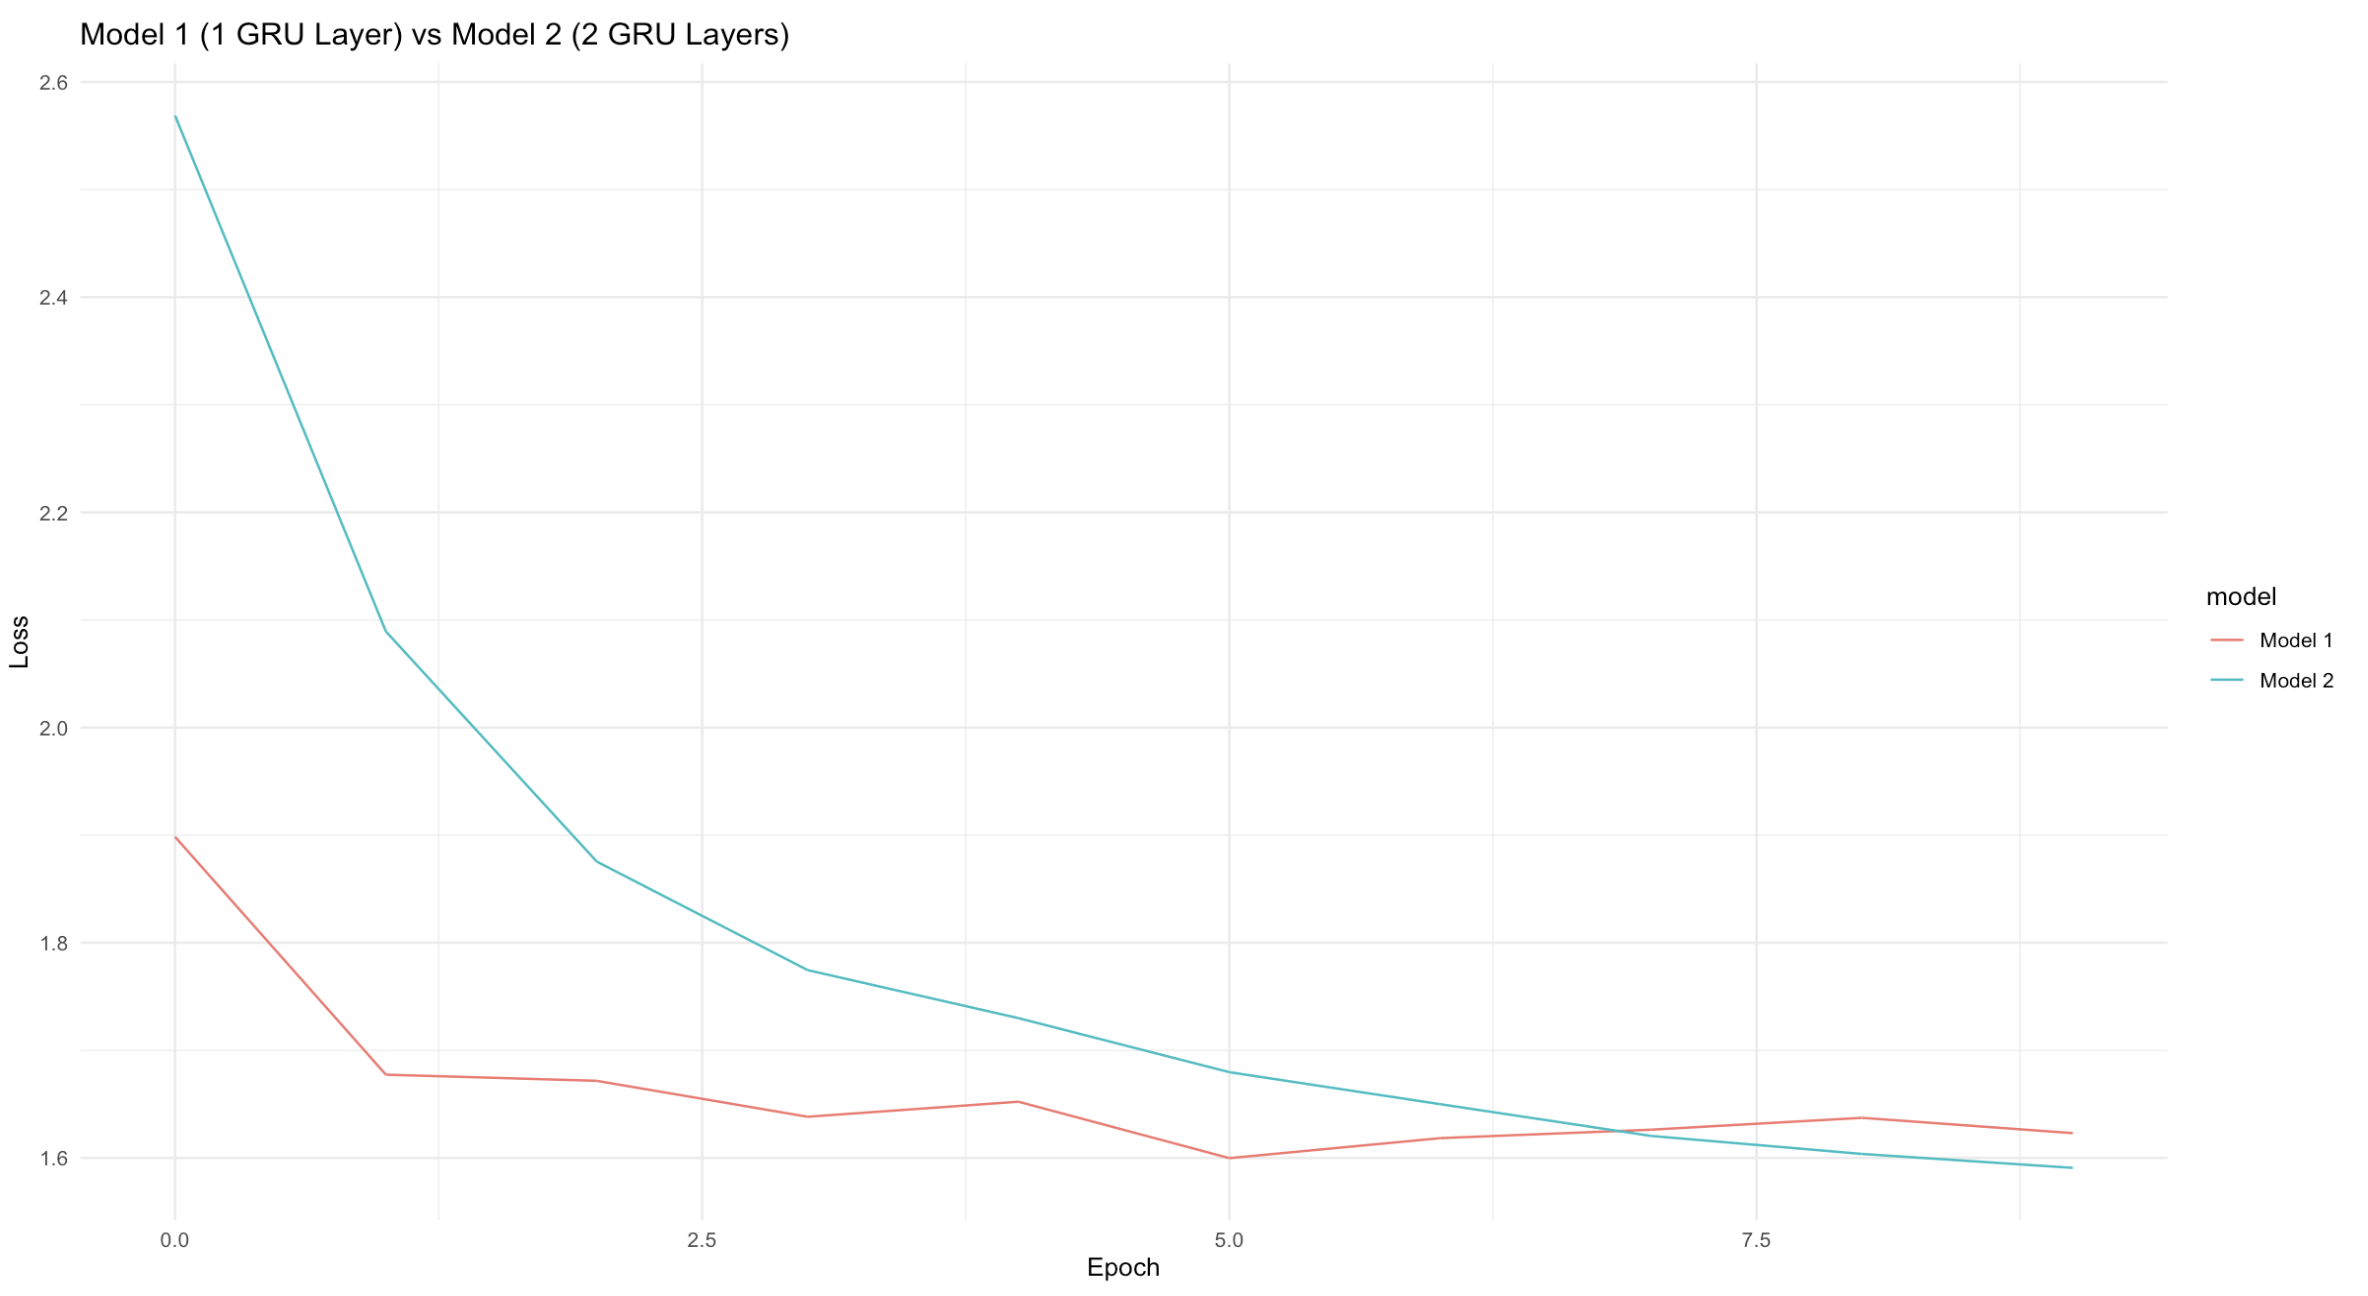
\includegraphics{"../Figures/Figure_4.png"}
\caption{Figure 4}
\end{figure}

\begin{figure}
\centering
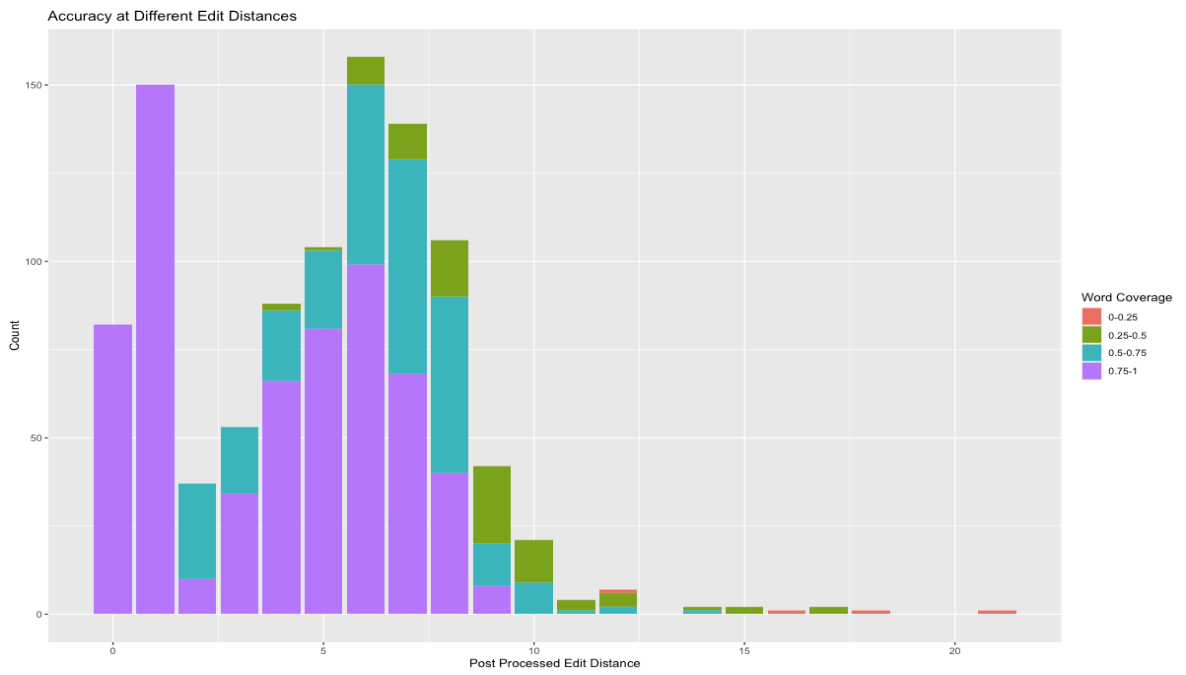
\includegraphics{"../Figures/Figure_5.png"}
\caption{Figure 5}
\end{figure}

\begin{figure}
\centering
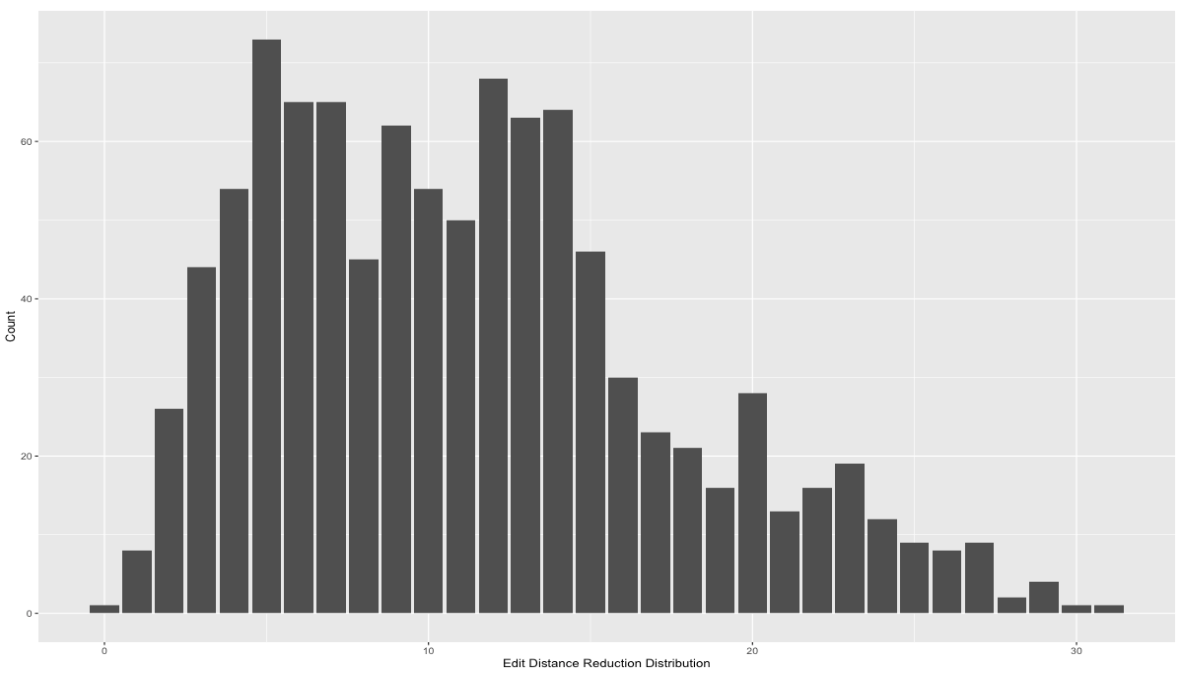
\includegraphics{"../Figures/Figure_6.png"}
\caption{Figure 6}
\end{figure}

\begin{figure}
\centering
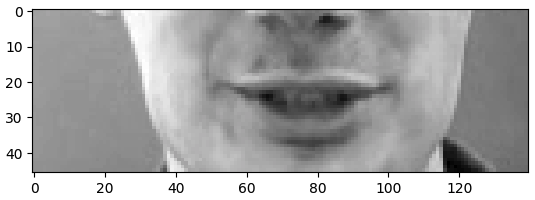
\includegraphics{"../Figures/Figure_7.png"}
\caption{Figure 7}
\end{figure}

\begin{figure}
\centering
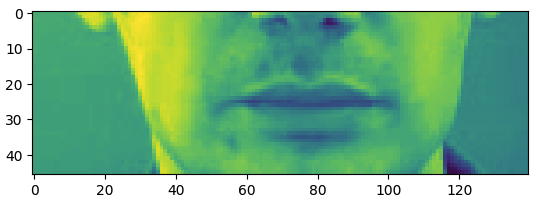
\includegraphics{"../Figures/Figure_8.png"}
\caption{Figure 8}
\end{figure}

\begin{figure}
\centering
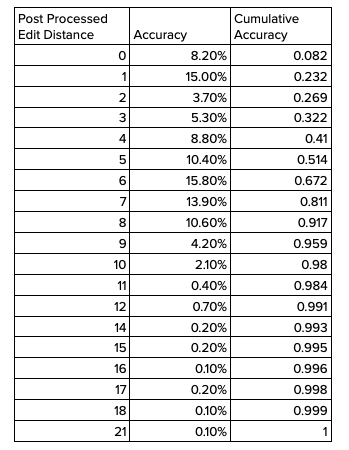
\includegraphics{"../Figures/Figure_9.png"}
\caption{Figure 9}
\end{figure}

\begin{figure}
\centering
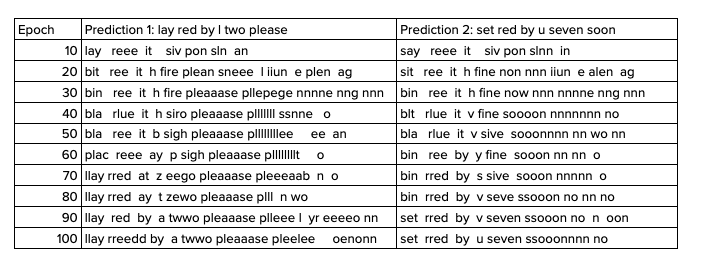
\includegraphics{"../Figures/Figure_10.png"}
\caption{Figure 10}
\end{figure}

\end{document}
